
% Default to the notebook output style

    


% Inherit from the specified cell style.




    
\documentclass[11pt]{article}

    
    
    \usepackage[T1]{fontenc}
    % Nicer default font than Computer Modern for most use cases
    \usepackage{palatino}

    % Basic figure setup, for now with no caption control since it's done
    % automatically by Pandoc (which extracts ![](path) syntax from Markdown).
    \usepackage{graphicx}
    % We will generate all images so they have a width \maxwidth. This means
    % that they will get their normal width if they fit onto the page, but
    % are scaled down if they would overflow the margins.
    \makeatletter
    \def\maxwidth{\ifdim\Gin@nat@width>\linewidth\linewidth
    \else\Gin@nat@width\fi}
    \makeatother
    \let\Oldincludegraphics\includegraphics
    % Set max figure width to be 80% of text width, for now hardcoded.
    \renewcommand{\includegraphics}[1]{\Oldincludegraphics[width=.8\maxwidth]{#1}}
    % Ensure that by default, figures have no caption (until we provide a
    % proper Figure object with a Caption API and a way to capture that
    % in the conversion process - todo).
    \usepackage{caption}
    \DeclareCaptionLabelFormat{nolabel}{}
    \captionsetup{labelformat=nolabel}

    \usepackage{adjustbox} % Used to constrain images to a maximum size 
    \usepackage{xcolor} % Allow colors to be defined
    \usepackage{enumerate} % Needed for markdown enumerations to work
    \usepackage{geometry} % Used to adjust the document margins
    \usepackage{amsmath} % Equations
    \usepackage{amssymb} % Equations
    \usepackage{textcomp} % defines textquotesingle
    % Hack from http://tex.stackexchange.com/a/47451/13684:
    \AtBeginDocument{%
        \def\PYZsq{\textquotesingle}% Upright quotes in Pygmentized code
    }
    \usepackage{upquote} % Upright quotes for verbatim code
    \usepackage{eurosym} % defines \euro
    \usepackage[mathletters]{ucs} % Extended unicode (utf-8) support
    \usepackage[utf8x]{inputenc} % Allow utf-8 characters in the tex document
    \usepackage{fancyvrb} % verbatim replacement that allows latex
    \usepackage{grffile} % extends the file name processing of package graphics 
                         % to support a larger range 
    % The hyperref package gives us a pdf with properly built
    % internal navigation ('pdf bookmarks' for the table of contents,
    % internal cross-reference links, web links for URLs, etc.)
    \usepackage{hyperref}
    \usepackage{longtable} % longtable support required by pandoc >1.10
    \usepackage{booktabs}  % table support for pandoc > 1.12.2
    \usepackage[normalem]{ulem} % ulem is needed to support strikethroughs (\sout)
                                % normalem makes italics be italics, not underlines
    

    
    
    % Colors for the hyperref package
    \definecolor{urlcolor}{rgb}{0,.145,.698}
    \definecolor{linkcolor}{rgb}{.71,0.21,0.01}
    \definecolor{citecolor}{rgb}{.12,.54,.11}

    % ANSI colors
    \definecolor{ansi-black}{HTML}{3E424D}
    \definecolor{ansi-black-intense}{HTML}{282C36}
    \definecolor{ansi-red}{HTML}{E75C58}
    \definecolor{ansi-red-intense}{HTML}{B22B31}
    \definecolor{ansi-green}{HTML}{00A250}
    \definecolor{ansi-green-intense}{HTML}{007427}
    \definecolor{ansi-yellow}{HTML}{DDB62B}
    \definecolor{ansi-yellow-intense}{HTML}{B27D12}
    \definecolor{ansi-blue}{HTML}{208FFB}
    \definecolor{ansi-blue-intense}{HTML}{0065CA}
    \definecolor{ansi-magenta}{HTML}{D160C4}
    \definecolor{ansi-magenta-intense}{HTML}{A03196}
    \definecolor{ansi-cyan}{HTML}{60C6C8}
    \definecolor{ansi-cyan-intense}{HTML}{258F8F}
    \definecolor{ansi-white}{HTML}{C5C1B4}
    \definecolor{ansi-white-intense}{HTML}{A1A6B2}

    % commands and environments needed by pandoc snippets
    % extracted from the output of `pandoc -s`
    \providecommand{\tightlist}{%
      \setlength{\itemsep}{0pt}\setlength{\parskip}{0pt}}
    \DefineVerbatimEnvironment{Highlighting}{Verbatim}{commandchars=\\\{\}}
    % Add ',fontsize=\small' for more characters per line
    \newenvironment{Shaded}{}{}
    \newcommand{\KeywordTok}[1]{\textcolor[rgb]{0.00,0.44,0.13}{\textbf{{#1}}}}
    \newcommand{\DataTypeTok}[1]{\textcolor[rgb]{0.56,0.13,0.00}{{#1}}}
    \newcommand{\DecValTok}[1]{\textcolor[rgb]{0.25,0.63,0.44}{{#1}}}
    \newcommand{\BaseNTok}[1]{\textcolor[rgb]{0.25,0.63,0.44}{{#1}}}
    \newcommand{\FloatTok}[1]{\textcolor[rgb]{0.25,0.63,0.44}{{#1}}}
    \newcommand{\CharTok}[1]{\textcolor[rgb]{0.25,0.44,0.63}{{#1}}}
    \newcommand{\StringTok}[1]{\textcolor[rgb]{0.25,0.44,0.63}{{#1}}}
    \newcommand{\CommentTok}[1]{\textcolor[rgb]{0.38,0.63,0.69}{\textit{{#1}}}}
    \newcommand{\OtherTok}[1]{\textcolor[rgb]{0.00,0.44,0.13}{{#1}}}
    \newcommand{\AlertTok}[1]{\textcolor[rgb]{1.00,0.00,0.00}{\textbf{{#1}}}}
    \newcommand{\FunctionTok}[1]{\textcolor[rgb]{0.02,0.16,0.49}{{#1}}}
    \newcommand{\RegionMarkerTok}[1]{{#1}}
    \newcommand{\ErrorTok}[1]{\textcolor[rgb]{1.00,0.00,0.00}{\textbf{{#1}}}}
    \newcommand{\NormalTok}[1]{{#1}}
    
    % Additional commands for more recent versions of Pandoc
    \newcommand{\ConstantTok}[1]{\textcolor[rgb]{0.53,0.00,0.00}{{#1}}}
    \newcommand{\SpecialCharTok}[1]{\textcolor[rgb]{0.25,0.44,0.63}{{#1}}}
    \newcommand{\VerbatimStringTok}[1]{\textcolor[rgb]{0.25,0.44,0.63}{{#1}}}
    \newcommand{\SpecialStringTok}[1]{\textcolor[rgb]{0.73,0.40,0.53}{{#1}}}
    \newcommand{\ImportTok}[1]{{#1}}
    \newcommand{\DocumentationTok}[1]{\textcolor[rgb]{0.73,0.13,0.13}{\textit{{#1}}}}
    \newcommand{\AnnotationTok}[1]{\textcolor[rgb]{0.38,0.63,0.69}{\textbf{\textit{{#1}}}}}
    \newcommand{\CommentVarTok}[1]{\textcolor[rgb]{0.38,0.63,0.69}{\textbf{\textit{{#1}}}}}
    \newcommand{\VariableTok}[1]{\textcolor[rgb]{0.10,0.09,0.49}{{#1}}}
    \newcommand{\ControlFlowTok}[1]{\textcolor[rgb]{0.00,0.44,0.13}{\textbf{{#1}}}}
    \newcommand{\OperatorTok}[1]{\textcolor[rgb]{0.40,0.40,0.40}{{#1}}}
    \newcommand{\BuiltInTok}[1]{{#1}}
    \newcommand{\ExtensionTok}[1]{{#1}}
    \newcommand{\PreprocessorTok}[1]{\textcolor[rgb]{0.74,0.48,0.00}{{#1}}}
    \newcommand{\AttributeTok}[1]{\textcolor[rgb]{0.49,0.56,0.16}{{#1}}}
    \newcommand{\InformationTok}[1]{\textcolor[rgb]{0.38,0.63,0.69}{\textbf{\textit{{#1}}}}}
    \newcommand{\WarningTok}[1]{\textcolor[rgb]{0.38,0.63,0.69}{\textbf{\textit{{#1}}}}}
    
    
    % Define a nice break command that doesn't care if a line doesn't already
    % exist.
    \def\br{\hspace*{\fill} \\* }
    % Math Jax compatability definitions
    \def\gt{>}
    \def\lt{<}
    % Document parameters
    \title{report}
    
    
    

    % Pygments definitions
    
\makeatletter
\def\PY@reset{\let\PY@it=\relax \let\PY@bf=\relax%
    \let\PY@ul=\relax \let\PY@tc=\relax%
    \let\PY@bc=\relax \let\PY@ff=\relax}
\def\PY@tok#1{\csname PY@tok@#1\endcsname}
\def\PY@toks#1+{\ifx\relax#1\empty\else%
    \PY@tok{#1}\expandafter\PY@toks\fi}
\def\PY@do#1{\PY@bc{\PY@tc{\PY@ul{%
    \PY@it{\PY@bf{\PY@ff{#1}}}}}}}
\def\PY#1#2{\PY@reset\PY@toks#1+\relax+\PY@do{#2}}

\expandafter\def\csname PY@tok@gd\endcsname{\def\PY@tc##1{\textcolor[rgb]{0.63,0.00,0.00}{##1}}}
\expandafter\def\csname PY@tok@gu\endcsname{\let\PY@bf=\textbf\def\PY@tc##1{\textcolor[rgb]{0.50,0.00,0.50}{##1}}}
\expandafter\def\csname PY@tok@gt\endcsname{\def\PY@tc##1{\textcolor[rgb]{0.00,0.27,0.87}{##1}}}
\expandafter\def\csname PY@tok@gs\endcsname{\let\PY@bf=\textbf}
\expandafter\def\csname PY@tok@gr\endcsname{\def\PY@tc##1{\textcolor[rgb]{1.00,0.00,0.00}{##1}}}
\expandafter\def\csname PY@tok@cm\endcsname{\let\PY@it=\textit\def\PY@tc##1{\textcolor[rgb]{0.25,0.50,0.50}{##1}}}
\expandafter\def\csname PY@tok@vg\endcsname{\def\PY@tc##1{\textcolor[rgb]{0.10,0.09,0.49}{##1}}}
\expandafter\def\csname PY@tok@vi\endcsname{\def\PY@tc##1{\textcolor[rgb]{0.10,0.09,0.49}{##1}}}
\expandafter\def\csname PY@tok@mh\endcsname{\def\PY@tc##1{\textcolor[rgb]{0.40,0.40,0.40}{##1}}}
\expandafter\def\csname PY@tok@cs\endcsname{\let\PY@it=\textit\def\PY@tc##1{\textcolor[rgb]{0.25,0.50,0.50}{##1}}}
\expandafter\def\csname PY@tok@ge\endcsname{\let\PY@it=\textit}
\expandafter\def\csname PY@tok@vc\endcsname{\def\PY@tc##1{\textcolor[rgb]{0.10,0.09,0.49}{##1}}}
\expandafter\def\csname PY@tok@il\endcsname{\def\PY@tc##1{\textcolor[rgb]{0.40,0.40,0.40}{##1}}}
\expandafter\def\csname PY@tok@go\endcsname{\def\PY@tc##1{\textcolor[rgb]{0.53,0.53,0.53}{##1}}}
\expandafter\def\csname PY@tok@cp\endcsname{\def\PY@tc##1{\textcolor[rgb]{0.74,0.48,0.00}{##1}}}
\expandafter\def\csname PY@tok@gi\endcsname{\def\PY@tc##1{\textcolor[rgb]{0.00,0.63,0.00}{##1}}}
\expandafter\def\csname PY@tok@gh\endcsname{\let\PY@bf=\textbf\def\PY@tc##1{\textcolor[rgb]{0.00,0.00,0.50}{##1}}}
\expandafter\def\csname PY@tok@ni\endcsname{\let\PY@bf=\textbf\def\PY@tc##1{\textcolor[rgb]{0.60,0.60,0.60}{##1}}}
\expandafter\def\csname PY@tok@nl\endcsname{\def\PY@tc##1{\textcolor[rgb]{0.63,0.63,0.00}{##1}}}
\expandafter\def\csname PY@tok@nn\endcsname{\let\PY@bf=\textbf\def\PY@tc##1{\textcolor[rgb]{0.00,0.00,1.00}{##1}}}
\expandafter\def\csname PY@tok@no\endcsname{\def\PY@tc##1{\textcolor[rgb]{0.53,0.00,0.00}{##1}}}
\expandafter\def\csname PY@tok@na\endcsname{\def\PY@tc##1{\textcolor[rgb]{0.49,0.56,0.16}{##1}}}
\expandafter\def\csname PY@tok@nb\endcsname{\def\PY@tc##1{\textcolor[rgb]{0.00,0.50,0.00}{##1}}}
\expandafter\def\csname PY@tok@nc\endcsname{\let\PY@bf=\textbf\def\PY@tc##1{\textcolor[rgb]{0.00,0.00,1.00}{##1}}}
\expandafter\def\csname PY@tok@nd\endcsname{\def\PY@tc##1{\textcolor[rgb]{0.67,0.13,1.00}{##1}}}
\expandafter\def\csname PY@tok@ne\endcsname{\let\PY@bf=\textbf\def\PY@tc##1{\textcolor[rgb]{0.82,0.25,0.23}{##1}}}
\expandafter\def\csname PY@tok@nf\endcsname{\def\PY@tc##1{\textcolor[rgb]{0.00,0.00,1.00}{##1}}}
\expandafter\def\csname PY@tok@si\endcsname{\let\PY@bf=\textbf\def\PY@tc##1{\textcolor[rgb]{0.73,0.40,0.53}{##1}}}
\expandafter\def\csname PY@tok@s2\endcsname{\def\PY@tc##1{\textcolor[rgb]{0.73,0.13,0.13}{##1}}}
\expandafter\def\csname PY@tok@nt\endcsname{\let\PY@bf=\textbf\def\PY@tc##1{\textcolor[rgb]{0.00,0.50,0.00}{##1}}}
\expandafter\def\csname PY@tok@nv\endcsname{\def\PY@tc##1{\textcolor[rgb]{0.10,0.09,0.49}{##1}}}
\expandafter\def\csname PY@tok@s1\endcsname{\def\PY@tc##1{\textcolor[rgb]{0.73,0.13,0.13}{##1}}}
\expandafter\def\csname PY@tok@ch\endcsname{\let\PY@it=\textit\def\PY@tc##1{\textcolor[rgb]{0.25,0.50,0.50}{##1}}}
\expandafter\def\csname PY@tok@m\endcsname{\def\PY@tc##1{\textcolor[rgb]{0.40,0.40,0.40}{##1}}}
\expandafter\def\csname PY@tok@gp\endcsname{\let\PY@bf=\textbf\def\PY@tc##1{\textcolor[rgb]{0.00,0.00,0.50}{##1}}}
\expandafter\def\csname PY@tok@sh\endcsname{\def\PY@tc##1{\textcolor[rgb]{0.73,0.13,0.13}{##1}}}
\expandafter\def\csname PY@tok@ow\endcsname{\let\PY@bf=\textbf\def\PY@tc##1{\textcolor[rgb]{0.67,0.13,1.00}{##1}}}
\expandafter\def\csname PY@tok@sx\endcsname{\def\PY@tc##1{\textcolor[rgb]{0.00,0.50,0.00}{##1}}}
\expandafter\def\csname PY@tok@bp\endcsname{\def\PY@tc##1{\textcolor[rgb]{0.00,0.50,0.00}{##1}}}
\expandafter\def\csname PY@tok@c1\endcsname{\let\PY@it=\textit\def\PY@tc##1{\textcolor[rgb]{0.25,0.50,0.50}{##1}}}
\expandafter\def\csname PY@tok@o\endcsname{\def\PY@tc##1{\textcolor[rgb]{0.40,0.40,0.40}{##1}}}
\expandafter\def\csname PY@tok@kc\endcsname{\let\PY@bf=\textbf\def\PY@tc##1{\textcolor[rgb]{0.00,0.50,0.00}{##1}}}
\expandafter\def\csname PY@tok@c\endcsname{\let\PY@it=\textit\def\PY@tc##1{\textcolor[rgb]{0.25,0.50,0.50}{##1}}}
\expandafter\def\csname PY@tok@mf\endcsname{\def\PY@tc##1{\textcolor[rgb]{0.40,0.40,0.40}{##1}}}
\expandafter\def\csname PY@tok@err\endcsname{\def\PY@bc##1{\setlength{\fboxsep}{0pt}\fcolorbox[rgb]{1.00,0.00,0.00}{1,1,1}{\strut ##1}}}
\expandafter\def\csname PY@tok@mb\endcsname{\def\PY@tc##1{\textcolor[rgb]{0.40,0.40,0.40}{##1}}}
\expandafter\def\csname PY@tok@ss\endcsname{\def\PY@tc##1{\textcolor[rgb]{0.10,0.09,0.49}{##1}}}
\expandafter\def\csname PY@tok@sr\endcsname{\def\PY@tc##1{\textcolor[rgb]{0.73,0.40,0.53}{##1}}}
\expandafter\def\csname PY@tok@mo\endcsname{\def\PY@tc##1{\textcolor[rgb]{0.40,0.40,0.40}{##1}}}
\expandafter\def\csname PY@tok@kd\endcsname{\let\PY@bf=\textbf\def\PY@tc##1{\textcolor[rgb]{0.00,0.50,0.00}{##1}}}
\expandafter\def\csname PY@tok@mi\endcsname{\def\PY@tc##1{\textcolor[rgb]{0.40,0.40,0.40}{##1}}}
\expandafter\def\csname PY@tok@kn\endcsname{\let\PY@bf=\textbf\def\PY@tc##1{\textcolor[rgb]{0.00,0.50,0.00}{##1}}}
\expandafter\def\csname PY@tok@cpf\endcsname{\let\PY@it=\textit\def\PY@tc##1{\textcolor[rgb]{0.25,0.50,0.50}{##1}}}
\expandafter\def\csname PY@tok@kr\endcsname{\let\PY@bf=\textbf\def\PY@tc##1{\textcolor[rgb]{0.00,0.50,0.00}{##1}}}
\expandafter\def\csname PY@tok@s\endcsname{\def\PY@tc##1{\textcolor[rgb]{0.73,0.13,0.13}{##1}}}
\expandafter\def\csname PY@tok@kp\endcsname{\def\PY@tc##1{\textcolor[rgb]{0.00,0.50,0.00}{##1}}}
\expandafter\def\csname PY@tok@w\endcsname{\def\PY@tc##1{\textcolor[rgb]{0.73,0.73,0.73}{##1}}}
\expandafter\def\csname PY@tok@kt\endcsname{\def\PY@tc##1{\textcolor[rgb]{0.69,0.00,0.25}{##1}}}
\expandafter\def\csname PY@tok@sc\endcsname{\def\PY@tc##1{\textcolor[rgb]{0.73,0.13,0.13}{##1}}}
\expandafter\def\csname PY@tok@sb\endcsname{\def\PY@tc##1{\textcolor[rgb]{0.73,0.13,0.13}{##1}}}
\expandafter\def\csname PY@tok@k\endcsname{\let\PY@bf=\textbf\def\PY@tc##1{\textcolor[rgb]{0.00,0.50,0.00}{##1}}}
\expandafter\def\csname PY@tok@se\endcsname{\let\PY@bf=\textbf\def\PY@tc##1{\textcolor[rgb]{0.73,0.40,0.13}{##1}}}
\expandafter\def\csname PY@tok@sd\endcsname{\let\PY@it=\textit\def\PY@tc##1{\textcolor[rgb]{0.73,0.13,0.13}{##1}}}

\def\PYZbs{\char`\\}
\def\PYZus{\char`\_}
\def\PYZob{\char`\{}
\def\PYZcb{\char`\}}
\def\PYZca{\char`\^}
\def\PYZam{\char`\&}
\def\PYZlt{\char`\<}
\def\PYZgt{\char`\>}
\def\PYZsh{\char`\#}
\def\PYZpc{\char`\%}
\def\PYZdl{\char`\$}
\def\PYZhy{\char`\-}
\def\PYZsq{\char`\'}
\def\PYZdq{\char`\"}
\def\PYZti{\char`\~}
% for compatibility with earlier versions
\def\PYZat{@}
\def\PYZlb{[}
\def\PYZrb{]}
\makeatother


    % Exact colors from NB
    \definecolor{incolor}{rgb}{0.0, 0.0, 0.5}
    \definecolor{outcolor}{rgb}{0.545, 0.0, 0.0}



    
    % Prevent overflowing lines due to hard-to-break entities
    \sloppy 
    % Setup hyperref package
    \hypersetup{
      breaklinks=true,  % so long urls are correctly broken across lines
      colorlinks=true,
      urlcolor=urlcolor,
      linkcolor=linkcolor,
      citecolor=citecolor,
      }
    % Slightly bigger margins than the latex defaults
    
    \geometry{verbose,tmargin=1in,bmargin=1in,lmargin=1in,rmargin=1in}
    
    

    \begin{document}
    
    

    
    

    
    \section{Machine Learning Engineer
Nanodegree}\label{machine-learning-engineer-nanodegree}

\subsection{Capstone Project}\label{capstone-project}

By Eakalak Suthampan\\December 12th, 2017

\section{WSDM - KKBox's Churn Prediction
Challenge}\label{wsdm---kkboxs-churn-prediction-challenge}

Can you predict when subscribers will churn?

\section{Definition}\label{definition}

\subsection{Project Overview}\label{project-overview}

Customer churn prediction is essential for businesses. Early prediction
of customers churn can help businesses to propose marketing campaign to
prevent their customers from canceling their subscription, product or
service. There are two broad approaches for churn analysis. Machine
learning which we will focus and
\href{https://en.wikipedia.org/wiki/Survival_analysis}{survival
analysis}. Machine learning methods, specifically classification, are
widely used due to their high performance and ability to handle complex
relationships in data. On the other hand, survival analyses can provide
value by answering a different set of questions. Quantities, such as
survival and hazard functions, can be used to forecast which customers
will churn in a particular time period.

This capstone will take the problem from the Kaggle competition
\href{https://www.kaggle.com/c/kkbox-churn-prediction-challenge}{``WSDM
- KKBox's Churn Prediction Challenge''}. The KKBOX is Asia's leading
music streaming service and would like to build an algorithm that
predicts whether a user will churn after their subscription expires.
Currently, the company uses survival analysis techniques to determine
the residual membership life time for each subscriber. By adopting
different methods, KKBOX anticipates they'll discover new insights to
why users leave so they can be proactive in keeping users dancing.

Some interesting practical works about churn prediction.
\href{http://daynebatten.com/2015/02/customer-churn-survival-analysis/}{Analyzing
Customer Churn -- Basic Survival Analysis} demonstrates to use R Code to
plot survival curve which shows relationship between days since
subscribing and percent surviving.
\href{https://docs.microsoft.com/en-us/azure/machine-learning/studio/azure-ml-customer-churn-scenario}{Analyzing
Customer Churn by using Azure Machine Learning} shows machine learning
approach using Azure for customer churn prediction. It used ensemble of
many classifiers such as Logistic Regression, Boosted Tree, Averaged
Perceptron, SVM to predict customer churn.

\subsection{Problem Statement}\label{problem-statement}

The objective for the Kaggle competition
\href{https://www.kaggle.com/c/kkbox-churn-prediction-challenge}{``WSDM
- KKBox's Churn Prediction Challenge''} is predicting whether a user
will churn after their subscription expires. \textbf{The criteria of
``churn'' is no new valid service subscription within 30 days after the
current membership expires.} I will build binary classification model to
predict whether a user will `churn' or `not churn' after their
subscription expires.

\subsection{Metrics}\label{metrics}

Since we would like to identify customer churn as much as possible (high
\href{https://machinelearningmastery.com/classification-accuracy-is-not-enough-more-performance-measures-you-can-use/}{recall})
while still getting acceptable
\href{https://machinelearningmastery.com/classification-accuracy-is-not-enough-more-performance-measures-you-can-use/}{precision}.
Therefore, I will use
\href{https://machinelearningmastery.com/classification-accuracy-is-not-enough-more-performance-measures-you-can-use/}{f1\_score}
as evaluation metric since the f1\_score conveys the balance between the
recall and the precision.

\[ F1 = 2 \cdot \frac{precision \cdot recall}{precision + recall} \]

\[ precision = \frac{tp}{tp + fp} \]

\[ recall = \frac{tp}{tp + fn} \]

By the way, the competition use
\href{https://www.kaggle.com/c/kkbox-churn-prediction-challenge\#evaluation}{binary
logloss} as evaluation metric. logloss is more precise to measure
classification performance because it is based on prediction in
probabilities. I think logloss is more appropriate when using in the
competition but I would like to use f1\_score because I think it is more
intuitive to explain to business in term of recall, precision. The
binary logloss equation is

\[ log loss = -\frac{1}{N}\sum_{i=1}^N {(y_i\log(p_i) + (1 - y_i)\log(1 - p_i))} \]

where $N$ is the number of observations, $log$ is the natural logarithm,
$y_{i}$ is the binary target, and $p_{i}$ is the predicted probability
that $y_{i}$ equals 1.

\section{Analysis}\label{analysis}

\subsection{Data Exploration}\label{data-exploration}

\subsubsection{Datasets}\label{datasets}

There are datasets as follows.

\begin{enumerate}
\def\labelenumi{\arabic{enumi}.}
\itemsep1pt\parskip0pt\parsep0pt
\item
  train.csv (44.5 MB, 992931 rows) is the train set. The train data
  consists of users whose subscription expires within the month of
  February 2017.

  \begin{itemize}
  \itemsep1pt\parskip0pt\parsep0pt
  \item
    msno: user id
  \item
    is\_churn: This is the target variable. Churn is defined as whether
    the user did not continue the subscription within 30 days of
    expiration. is\_churn = 1 means churn,is\_churn = 0 means renewal.
  \end{itemize}
\item
  sample\_submission\_zero.csv (43.5 MB, 970960 rows) is the test set.
  The test data is with users whose subscription expires within the
  month of March 2017.

  \begin{itemize}
  \itemsep1pt\parskip0pt\parsep0pt
  \item
    msno: user id
  \item
    is\_churn: This is what you will predict. Churn is defined as
    whether the user did not continue the subscription within 30 days of
    expiration. is\_churn = 1 means churn,is\_churn = 0 means renewal.
  \end{itemize}
\item
  transactions.csv (1.61 GB, 21547746 rows) is transactions of users up
  until 2/28/2017.

  \begin{itemize}
  \itemsep1pt\parskip0pt\parsep0pt
  \item
    msno: user id
  \item
    payment\_method\_id: payment method
  \item
    payment\_plan\_days: length of membership plan in days
  \item
    plan\_list\_price: in New Taiwan Dollar (NTD)
  \item
    actual\_amount\_paid: in New Taiwan Dollar (NTD)
  \item
    is\_auto\_renew
  \item
    transaction\_date: format \%Y\%m\%d
  \item
    membership\_expire\_date: format \%Y\%m\%d
  \item
    is\_cancel: whether or not the user canceled the membership in this
    transaction.
  \end{itemize}
\item
  user\_logs.csv (28.4 GB, 392106543 rows) describing listening
  behaviors of a user. Data collected until 2/28/2017.

  \begin{itemize}
  \itemsep1pt\parskip0pt\parsep0pt
  \item
    msno: user id
  \item
    date: format \%Y\%m\%d
  \item
    num\_25: \# of songs played less than 25\% of the song length
  \item
    num\_50: \# of songs played between 25\% to 50\% of the song length
  \item
    num\_75: \# of songs played between 50\% to 75\% of of the song
    length
  \item
    num\_985: \# of songs played between 75\% to 98.5\% of the song
    length
  \item
    num\_100: \# of songs played over 98.5\% of the song length
  \item
    num\_unq: \# of unique songs played
  \item
    total\_secs: total seconds played
  \end{itemize}
\item
  members.csv (352 MB, 5116194 rows) consist of user information. Note
  that not every user in the dataset is available.

  \begin{itemize}
  \itemsep1pt\parskip0pt\parsep0pt
  \item
    msno
  \item
    city
  \item
    bd: age. Note: this column has outlier values ranging from -7000 to
    2015, please use your judgement.
  \item
    gender: this column has NULL values
  \item
    registered\_via: registration method
  \item
    registration\_init\_time: format \%Y\%m\%d
  \item
    expiration\_date: format \%Y\%m\%d, taken as a snapshot at which the
    member.csv is extracted. Not representing the actual churn behavior.
  \end{itemize}
\end{enumerate}

There are additional datasets that were added later because the version
1 testing dataset (sample\_submission\_zero.csv) were leaked. So Kaggle
provided the new version 2 test dataset and more training sets as
folows.

\begin{enumerate}
\def\labelenumi{\arabic{enumi}.}
\setcounter{enumi}{5}
\itemsep1pt\parskip0pt\parsep0pt
\item
  sample\_submission\_v2.csv (40.6 MB) is the new test dataset for
  April, 2017. (replaced sample\_submission\_zero.csv)
\item
  train\_v2.csv (43.5 MB) contains additional churn data for March,
  2017.
\item
  transactions\_v2.csv (110 MB) contains additional transactions data
  until 3/31/2017.
\item
  user\_logs\_v2.csv (1.33 GB) contains additional user logs data until
  3/31/2017.
\item
  members\_v3.csv (408 MB) is the new member dataset. (replaced
  members.csv)
\end{enumerate}

for more information about the datasets please see at the Kaggle
competition
\href{https://www.kaggle.com/c/kkbox-churn-prediction-challenge}{``WSDM
- KKBox's Churn Prediction Challenge''}.

\subsubsection{Feature Engineering}\label{feature-engineering}

I managed to create the following new features from transactions.csv.

\begin{itemize}
\itemsep1pt\parskip0pt\parsep0pt
\item
  last transaction for each user: I guess that features such as
  payment\_method\_id, payment\_plan\_days, is\_auto\_renew,
  membership\_expire\_date, is\_cancel may effect the churn.
\item
  subscribe duration: If users have been subscribed for a long time,
  they should have less chance to churn.
\item
  oldest transaction date for each user: Some users may have very oldest
  transaction date but a short subscribe duration.
\item
  count of transactions for each user: may be the more transactions, the
  less likely to churn.
\end{itemize}

I managed to create the following new features from user\_logs.csv.

\begin{itemize}
\itemsep1pt\parskip0pt\parsep0pt
\item
  aggregate values such as total seconds played, total songs played for
  each user may effect the churn.
\item
  count of all logs for each user. This can tell number of activities
  for a user.
\item
  count of logs for the last 1 month for each user. If users don't have
  much activities in the last month (small log counts) they might have
  more chance to churn.
\end{itemize}

Finally, I merge all above features to the members.csv. Informations in
the members.csv such as user age and registration method may effect the
churn. For all merging, I use left join to merge features so there are
NAN values for records that cannot be merged.

    \subsubsection{Training dataset
information}\label{training-dataset-information}

    \begin{Verbatim}[commandchars=\\\{\}]
<class 'pandas.core.frame.DataFrame'>
RangeIndex: 1963891 entries, 0 to 1963890
Data columns (total 27 columns):
msno                       object
is\_churn                   int64
payment\_method\_id          int64
payment\_plan\_days          int64
plan\_list\_price            int64
actual\_amount\_paid         int64
is\_auto\_renew              int64
transaction\_date           int64
membership\_expire\_date     int64
is\_cancel                  int64
subscribe\_days             float64
oldest\_transaction\_date    int64
transaction\_count          float64
num\_25                     float64
num\_50                     float64
num\_75                     float64
num\_985                    float64
num\_100                    float64
num\_unq                    float64
total\_secs                 float64
log\_count\_all              float64
log\_count\_1\_month          float64
city                       float64
bd                         float64
gender                     object
registered\_via             float64
registration\_init\_time     float64
dtypes: float64(15), int64(10), object(2)
memory usage: 404.5+ MB
None

    \end{Verbatim}

    \subsection{Exploratory Visualization}\label{exploratory-visualization}

\subsubsection{Labels Count}\label{labels-count}

First, let see the counts of labels. You can see that the labels are
very imbalanced. The count of `is\_churn'=1 (churn) is very less than
`is\_churn'=0 (not churn). The prediction model may be biasd to the
majority which is not churn.

    \begin{center}
    \adjustimage{max size={0.9\linewidth}{0.9\paperheight}}{report_files/report_15_0.png}
    \end{center}
    { \hspace*{\fill} \\}
    
    \subsubsection{Count of NAN Values}\label{count-of-nan-values}

There are NAN values for the merged train dataset. The gender column has
NAN as majority value. The other columns have NAN values because I used
left join and some users don't have associate data in users\_log.csv and
members.csv.

    \begin{center}
    \adjustimage{max size={0.9\linewidth}{0.9\paperheight}}{report_files/report_17_0.png}
    \end{center}
    { \hspace*{\fill} \\}
    
    \subsubsection{Count of transactions}\label{count-of-transactions}

Vilolin plot for the count of transactions for each user shows that
lower transaction counts have higher probabilities to churn
(is\_churn=1) while higher transaction counts have higher probabilities
to not churn (is\_churn=0). There are many outliers for the
`is\_churn=1' (long tail).

    \begin{center}
    \adjustimage{max size={0.9\linewidth}{0.9\paperheight}}{report_files/report_19_0.png}
    \end{center}
    { \hspace*{\fill} \\}
    
    \subsubsection{is\_auto\_renew,
is\_cancel}\label{isux5fautoux5frenew-isux5fcancel}

Show count plot for `is\_auto\_renew' and `is\_cancel'. The plots show
that `is\_cancel=1' has high effect for user to churn while
`is\_auto\_renew=1' has very high effect for user to not churn.

    \begin{center}
    \adjustimage{max size={0.9\linewidth}{0.9\paperheight}}{report_files/report_21_0.png}
    \end{center}
    { \hspace*{\fill} \\}
    
    \begin{center}
    \adjustimage{max size={0.9\linewidth}{0.9\paperheight}}{report_files/report_22_0.png}
    \end{center}
    { \hspace*{\fill} \\}
    
    \subsubsection{Count of last month logs}\label{count-of-last-month-logs}

The count of last month logs means how much activities for user in the
last month. From the plot, `is\_churn=1' has higher occurrence at both
the top and bottom of the plot while `is\_churn=0' has very high
occurrence at the top of the plot.

    \begin{center}
    \adjustimage{max size={0.9\linewidth}{0.9\paperheight}}{report_files/report_24_0.png}
    \end{center}
    { \hspace*{\fill} \\}
    
    \subsection{Algorithms and Techniques}\label{algorithms-and-techniques}

First, before discussing about algorithms let's summarize the
characteristics of the train data.

\begin{itemize}
\itemsep1pt\parskip0pt\parsep0pt
\item
  very imbalanced label (churn data is very small compared to not churn
  data).
\item
  have a lot of missing values.
\item
  many columns have outlier values.
\item
  all columns are numeric or make sense to be numeric (for example,
  transaction\_date, membership\_expire\_date).
\end{itemize}

From the characteristics of the dataset, I think ensemble method such as
Random Forest and XGBoost are the most appropriate.

\begin{itemize}
\itemsep1pt\parskip0pt\parsep0pt
\item
  Random Forest uses bagging while XGBoost uses boosting to handle the
  imbalanced classification.\\
\item
  They don't need to do preprocessing steps like scaling and
  standardize.
\item
  They can handle the missing values.
\item
  XGBoost may be better in term of accuracy but need more parameter
  tuning than Random Forest.
\item
  Random Forest may be better in term of less overfitting if there are
  outlier values.
\item
  Randome Forest can use both numeric and category data while XGBoost
  can use only numeric data.
\end{itemize}

Random Forest is a bagging ensemble method working by training multiple
decision tree models on different samples (with replacement) and
different random features then average their predictions.

\[  \hat{y}=\frac{1}{N}\sum_{k=1}^N f_k(x_i) \]

where $f_k$ is a random features decision tree classifier and $x_i$ is a
random samples with replacement from training data and $N$ is number of
decision tree classifier. It aim to decrease variance not bias. This
\href{https://people.cs.pitt.edu/~milos/courses/cs2750-Spring04/lectures/class23.pdf}{lecture}
describes how it can reduce variance without changing bias.

Assume we measure a random variable $x$ with a $N(\mu,\sigma)$
distribution. If random variable $x$ is measured $k$ times
$(x_1,x_2,...x_k)$ and the value is estimated as:
$\frac{1}{k}(x_1+x_2+…+x_k)$.

\begin{itemize}
\itemsep1pt\parskip0pt\parsep0pt
\item
  Mean of the estimate is still $\mu$
\item
  But, variance is smaller
  $\frac{1}{k^2}(Var(x_1)+…Var(x_k)) = \frac{k\sigma^2}{k^2} = \frac{\sigma^2 }{k}$
\end{itemize}

XGBoost is a boosting ensemble method working by starting with a very
simple decision tree model (accuracy just slightly better than 50\%)
then incrementally training each new decision tree model instance to
emphasize the training instances that previous model misclassified then
use majority voting of these boosting models. Equation for
\href{http://xgboost.readthedocs.io/en/latest/model.html\#additive-training}{additive
training} (fix what we have learned, and add one new tree at a time) is

\[\hat{y}_i^{(t)} = \sum_{k=1}^t f_k(x_i)= \hat{y}_i^{(t-1)} + f_t(x_i)\]

where $\hat{y}_i^{(t)}$ is a prediction value at step $t$ and $f_t$ is a
new decision tree at step $t$ and $x_i$ is samples from the distribution
that weighted the misclassified instances from the previous step.
XGBoost aim to decrease bias, not variance.

    \subsection{Benchmark}\label{benchmark}

I will use two simple benchmarks as follows

\begin{itemize}
\itemsep1pt\parskip0pt\parsep0pt
\item
  use Dicision Tree as simple model benchmark to be compared with the
  Random Forest and XGBoost.
\item
  use a simple rule, if a user has no activities in the last 30 days
  then predict the user as churn.
\end{itemize}

    \section{Methodology}\label{methodology}

\subsection{Data Preprocessing}\label{data-preprocessing}

I will do the following data preprocessing.

\begin{itemize}
\itemsep1pt\parskip0pt\parsep0pt
\item
  convert column gender from category to be numeric (1=male, 2=female)
  because XGBoost need all features to be numeric.
\item
  drop msno column which is user id (does not need user id when training
  model).
\item
  Most of NAN values occured because using left join so I think it make
  sense to fill NAN with 0.
\end{itemize}

XGBoost and Random Forest don't need other feature transformations such
as scaling or standardizing.

    \subsection{Implementation}\label{implementation}

I will do following for tuning the initial models.

\begin{itemize}
\itemsep1pt\parskip0pt\parsep0pt
\item
  split 10\% of train data to be the test data. This will be used for
  comparing models.
\item
  train and compare two models, Random Forest and XGBoost.
\item
  tune model parameters using GridSearchCV (using small samples and
  small n\_estimates for training speed).
\end{itemize}

\subsubsection{XGBoost}\label{xgboost}

I will fixing the following parameters for GridSearchCV.

\begin{itemize}
\itemsep1pt\parskip0pt\parsep0pt
\item
  n\_estimators = 50 (using large n\_estimators will take very long time
  to run)
\item
  using 100000 records of the train data. (about 5\% of train data)
\item
  cv = 4 (cross validate)
\item
  scoring = `log\_loss' (since Kaggle use log\_loss as evaluation
  metric)
\item
  objective=`binary:logistic' (binary classification)
\end{itemize}

I will tune the following parameters using GridSearchCV.

\begin{itemize}
\itemsep1pt\parskip0pt\parsep0pt
\item
  ``max\_depth'': Maximum tree depth for base learners.
\item
  ``min\_child\_weight'': Minimum sum of instance weight(hessian) needed
  in a child.
\item
  ``subsample'': Subsample ratio of the training instance.
\item
  ``colsample\_bytree'': Subsample ratio of columns when constructing
  each tree.
\end{itemize}

the parameters range to tune are as follows.

\begin{itemize}
\itemsep1pt\parskip0pt\parsep0pt
\item
  ``max\_depth'': {[}4,5,6,7{]}
\item
  ``min\_child\_weight'' :{[}1,2,3{]}
\item
  ``subsample'': {[}0.6,1.0{]}
\item
  ``colsample\_bytree'': (0.6,1.0)\}
\end{itemize}

    The best parameters from GridSearchCV are

            \begin{Verbatim}[commandchars=\\\{\}]
{\color{outcolor}Out[{\color{outcolor}22}]:} \{'colsample\_bytree': 1.0,
          'max\_depth': 6,
          'min\_child\_weight': 1,
          'subsample': 0.6\}
\end{Verbatim}
        
    The first tuning scores on the train data are

    \begin{Verbatim}[commandchars=\\\{\}]
log\_loss = 0.0744267875661, recall = 0.757172395968, f1\_score = 0.809142383649

    \end{Verbatim}

    The first tuning scores on the test data are

    \begin{Verbatim}[commandchars=\\\{\}]
log\_loss = 0.0793903277045, recall = 0.71131547381, f1\_score = 0.766039902397

    \end{Verbatim}

    \subsubsection{Random Forest}\label{random-forest}

I will fixing the following parameters for GridSearchCV.

\begin{itemize}
\itemsep1pt\parskip0pt\parsep0pt
\item
  n\_estimators = 50 (using large n\_estimators will take very long time
  to run)
\item
  using 100000 records of the train data (about 5\% of train data).
\item
  cv = 4 (cross validate)
\item
  scoring = `log\_loss' (since Kaggle use log\_loss as evaluation
  metric)
\end{itemize}

I will tune the following parameters using GridSearchCV.

\begin{itemize}
\itemsep1pt\parskip0pt\parsep0pt
\item
  max\_features: The number of features to consider when looking for the
  best split.
\item
  max\_depth: The maximum depth of the tree.
\item
  min\_samples\_leaf: The minimum number of samples required to be at a
  leaf node.
\item
  min\_samples\_split: The minimum number of samples required to split
  an internal node.
\end{itemize}

the parameters range to tune are as follows.

\begin{itemize}
\itemsep1pt\parskip0pt\parsep0pt
\item
  ``max\_depth'': {[}4,5,6{]}
\item
  ``min\_samples\_split'' :{[}2,3,4{]}
\item
  ``min\_samples\_leaf'': {[}1,3,5{]}
\item
  ``max\_features'': (4,5,6)
\end{itemize}

I intent to tune Random Forest to less overfit than XGBoost to compare
results when submiting to Kaggle.

    The best parameters from GridSearchCV are

            \begin{Verbatim}[commandchars=\\\{\}]
{\color{outcolor}Out[{\color{outcolor}26}]:} \{'max\_depth': 6,
          'max\_features': 6,
          'min\_samples\_leaf': 1,
          'min\_samples\_split': 4\}
\end{Verbatim}
        
    The first scores on the train data are

    \begin{Verbatim}[commandchars=\\\{\}]
log\_loss = 0.0867531737872, recall = 0.719048849832, f1\_score = 0.777692361451

    \end{Verbatim}

    The first scores on the test data are

    \begin{Verbatim}[commandchars=\\\{\}]
log\_loss = 0.0879615918596, recall = 0.703851792616, f1\_score = 0.762709416522

    \end{Verbatim}

    Complications during the implementation are

\begin{itemize}
\itemsep1pt\parskip0pt\parsep0pt
\item
  GridSearchCV takes very long time to brute force searching the best
  parameters. So I need to use just small samples of the training data.
  The parameter `n\_estimator' also has a huge effect to the running
  time of GridSearchCV.
\item
  There are so many parameters for the algorithms but I can not fine
  tune them because adding one more choice of the parameter can add
  multiplication in the time consuming so it's hard to decide which
  parameters and how much of its range need to be tuned. May be I should
  consider RandomSearchCV instead of GridSearchCV for the next time.
\item
  For tuning Random Forest, increasing values for `max\_depth' and
  `max\_features' will get better score on the test data but I've found
  that it will overfit when submiting results to Kaggle.
\end{itemize}

    \subsection{Refinement}\label{refinement}

For final tuning, I will use parameters from the previous GridSearchCV
and do following to tune the final scores.

\begin{itemize}
\itemsep1pt\parskip0pt\parsep0pt
\item
  increase n\_estimates to be 500 for both XGBoost and Random Forest.
\item
  train on the full train data.
\item
  use the same test data as previous phase.
\end{itemize}

\subsubsection{XGBoost}\label{xgboost}

The final scores on the test data are

    \begin{Verbatim}[commandchars=\\\{\}]
log\_loss = 0.0747653657696, recall = 0.726042916167, f1\_score = 0.770590939633

    \end{Verbatim}

    \subsubsection{Random Forest}\label{random-forest}

The final scores on the test data are

    \begin{Verbatim}[commandchars=\\\{\}]
log\_loss = 0.0878255092431, recall = 0.711781953885, f1\_score = 0.764785908635

    \end{Verbatim}

    \subsubsection{Scores Summary}\label{scores-summary}

Compare scores for intermediate tuning on both train and test data and
final tuning on test data.

for XGBoost

    \begin{longtable}[c]{@{}llll@{}}
\toprule\addlinespace
metrics & first\_score\_on\_train\_data & first\_score\_on\_test\_data &
final\_score\_on\_test\_data
\\\addlinespace
\midrule\endhead
log\_loss & 0.07442678756606426 & 0.07939032770447087 &
0.07476536576963773
\\\addlinespace
recall & 0.7571723959679504 & 0.7113154738104758 & 0.7260429161668666
\\\addlinespace
f1\_score & 0.8091423836486672 & 0.7660399023970144 & 0.770590939632917
\\\addlinespace
\bottomrule
\end{longtable}

    
    for Random Forest

    \begin{longtable}[c]{@{}llll@{}}
\toprule\addlinespace
metrics & first\_score\_on\_train\_data & first\_score\_on\_test\_data &
final\_score\_on\_test\_data
\\\addlinespace
\midrule\endhead
log\_loss & 0.08675317378719496 & 0.08796159185956462 &
0.08782550924311255
\\\addlinespace
recall & 0.7190488498319979 & 0.7038517926162868 & 0.7117819538851127
\\\addlinespace
f1\_score & 0.7776923614508351 & 0.7627094165222416 & 0.7647859086352571
\\\addlinespace
\bottomrule
\end{longtable}

    
    For both XGBoost and Random Forest, the scores on both train and test
data are very close and seem not overfit. XGBoost final results on the
test data have better scores than Random Forest.

    \section{Results}\label{results}

\subsection{Model Evaluation and
Validation}\label{model-evaluation-and-validation}

I submitted results from both XGBoost and Random Forest to Kaggle. The
best result is from Random Forest model which I got 55th place out of
434 (top 13\%) on the Kaggle public leaderboard (As of DEC 7, 2017).

\begin{figure}[htbp]
\centering
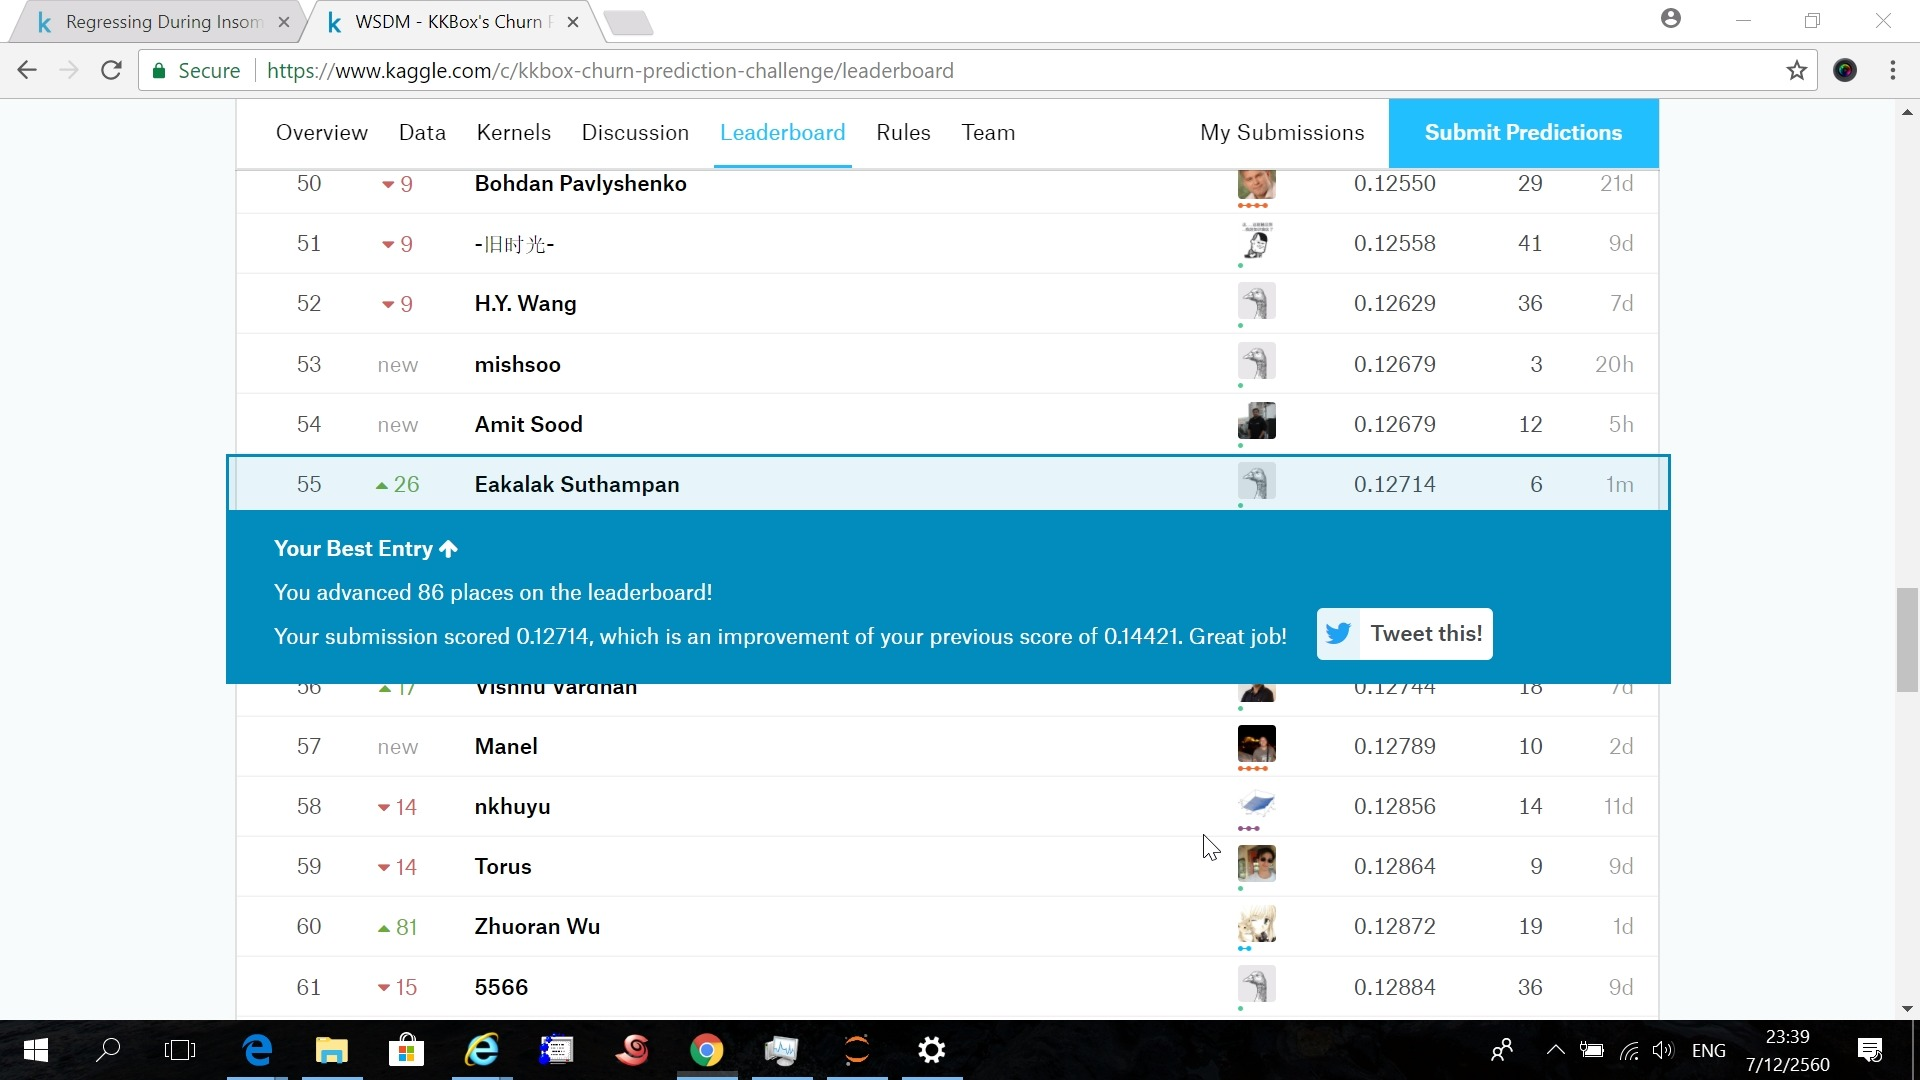
\includegraphics{lb.jpg}
\end{figure}

    \begin{longtable}[c]{@{}lll@{}}
\toprule\addlinespace
Model & log\_loss\_on\_Kaggle\_public\_leaderboard &
log\_loss\_on\_the\_test\_data
\\\addlinespace
\midrule\endhead
XGBoost & 0.14421 & 0.07476536576963773
\\\addlinespace
Random Forest & 0.12714 & 0.08782550924311255
\\\addlinespace
\bottomrule
\end{longtable}

    
    It's surprised me that Random Forest got higher score on Kaggle Public
Leaderboard although XGBoost got higher score on the test data. It seems
that both models are overfit to the real data but Random Forest is less
overfit than XGBoost. I think the reason that Random Forest is less
overfit is because both model have the parameter `maxdepth' equally
which is 6 so Random Forest which is bagging seem to less overfit than
XGBoost which is boosting.

So my final chosen model is Random Forest because in real life many of
user churn may don't have exact pattern so the less overfit model should
be better.

    \subsection{Justification}\label{justification}

I have the following benchmarks.

\begin{itemize}
\itemsep1pt\parskip0pt\parsep0pt
\item
  benchmark1: use a simple decision tree.
\item
  benchmark2: use a simple rule if user does not have usage log in the
  last month then predict user to churn.
\end{itemize}

Here are results of bechmarks to compare with the final chosen model.

    \begin{longtable}[c]{@{}llll@{}}
\toprule\addlinespace
model & log\_loss & recall & f1\_score
\\\addlinespace
\midrule\endhead
benchmark1 & 1.72517900298467 & 0.6258829801412769 & 0.6398909896099473
\\\addlinespace
benchmark2 & 8.747856170892863 & 0.413567906170865 & 0.1997039516025228
\\\addlinespace
Random Forest & 0.08782550924311255 & 0.7117819538851127 &
0.7647859086352571
\\\addlinespace
\bottomrule
\end{longtable}

    
    \begin{itemize}
\itemsep1pt\parskip0pt\parsep0pt
\item
  benchmark1 and benchmark2 cannot predict in probabilities so their
  log\_loss are very high.
\item
  benchmark1 has both recall and f1\_core significantly lower than
  Random Forest.
\item
  benchmark2 has both recall and f1\_core significantly lower than
  Random Forest. Especially the very low f1\_score compared to recall
  tells that it has very low precision (high False Positive).
\item
  Random Forest has high enough scores on both recall and f1\_score
  which means it can effectively identify around 71 out of 100 for the
  churn users while still maintain acceptable false alarm.
\end{itemize}

    \section{Conclusion}\label{conclusion}

\subsection{Free-Form Visualization}\label{free-form-visualization}

    \begin{center}
    \adjustimage{max size={0.9\linewidth}{0.9\paperheight}}{report_files/report_67_0.png}
    \end{center}
    { \hspace*{\fill} \\}
    
    Feature importances plot shows that `membership\_expire\_date',
`transaction\_date' and `is\_cancel' are the top 3 most important
features to predict customer churn. Most of important features are from
transactions.csv. Features from user\_log.csv and members.csv are almost
no importance.

    \subsection{Reflection}\label{reflection}

This project is an imbalanced binary classification problem. Kaggle
provides so many large datasets and so many features and I need to merge
these datasets together to derive some new useful features. This feature
engineering step is very time consuming for me and it consumed almost
all of 32GB of my RAM. After that I need to do data exploration and
visualization to understand more on the data. In the preprocessing step,
I need to clean the NAN values by just simply filling them with zero and
drop some columns that not meaningful to train model.

I choose ensemble tree based model Random Forest and XGBoost as they are
effective technique to
\href{https://www.analyticsvidhya.com/blog/2017/03/imbalanced-classification-problem/}{handle
imbalanced classification}. For evaluation metrics, Kaggle uses logloss
for this problem and I also use f1 along with recall as they can explain
to business in term of how many user churn can be identified and how
many false alarms.

For the train phase, I trained two model XGBoost and Random Forest. I
use GridSearchCV to fine tune the best parameters. This phase is also a
very time comsuming since GridSearchCV is a brute force method and the
training data are quite large. The scores on the train and test data are
quite similar and seem not overfit. XGBoost is better. It got around
0.07-0.08 for the logloss on the test data while Random Forest got
around 0.08-0.09. These scores are very much far better than the simple
rule based benchmark (if user has no activity longer than 30 days then
predict as churn) and non ensemble method benchmark like decision tree.

I submitted results from both XGBoost and Random Forest to Kaggle and
it's surprised me that Random Forest got very much better scores on the
Kaggle Public Learderboard although XGBoost score is better on my test
data. I got around 55th place out of 434 (top 13\%) for the Random
Forest as the day I submitted. Random Forest logloss score on the Kaggle
Public Learderboard is around 0.12 while XGBoost is around 0.14. Both
models seem to be overfit when compare to the score on my test data.

\subsection{Improvement}\label{improvement}

To improve the model I will focus on reducing overfit.

\begin{itemize}
\itemsep1pt\parskip0pt\parsep0pt
\item
  Explore and filter out more outlier values.
\item
  Remove unnecessary features based on the feature importances plot.
\item
  Tuning parameters that effect the overfit such as reducing maxdepth.
\item
  Try early stoping technique in XGBoost which can help preventing
  overfit.
\item
  Train with more data if possible to make model more generalize.
\item
  Try to create new feature that does not depend on date value and not
  strong correlate with the existing features.
\item
  Ensemble result of both XGBoost and Random Forest.
\end{itemize}


    % Add a bibliography block to the postdoc
    
    
    
    \end{document}
